\chapter{Practical}
\section{A-Level Trend}
\begin{itemize}
    \item One question on electrical circuits.
    \item One question on oscillations.
    \item One `wild card' question on any topic.
    \item One planning question on any topic.
\end{itemize}
\section{Measurements \& Calculations}
\begin{itemize}
    \begin{figure}[H]
        \centering
        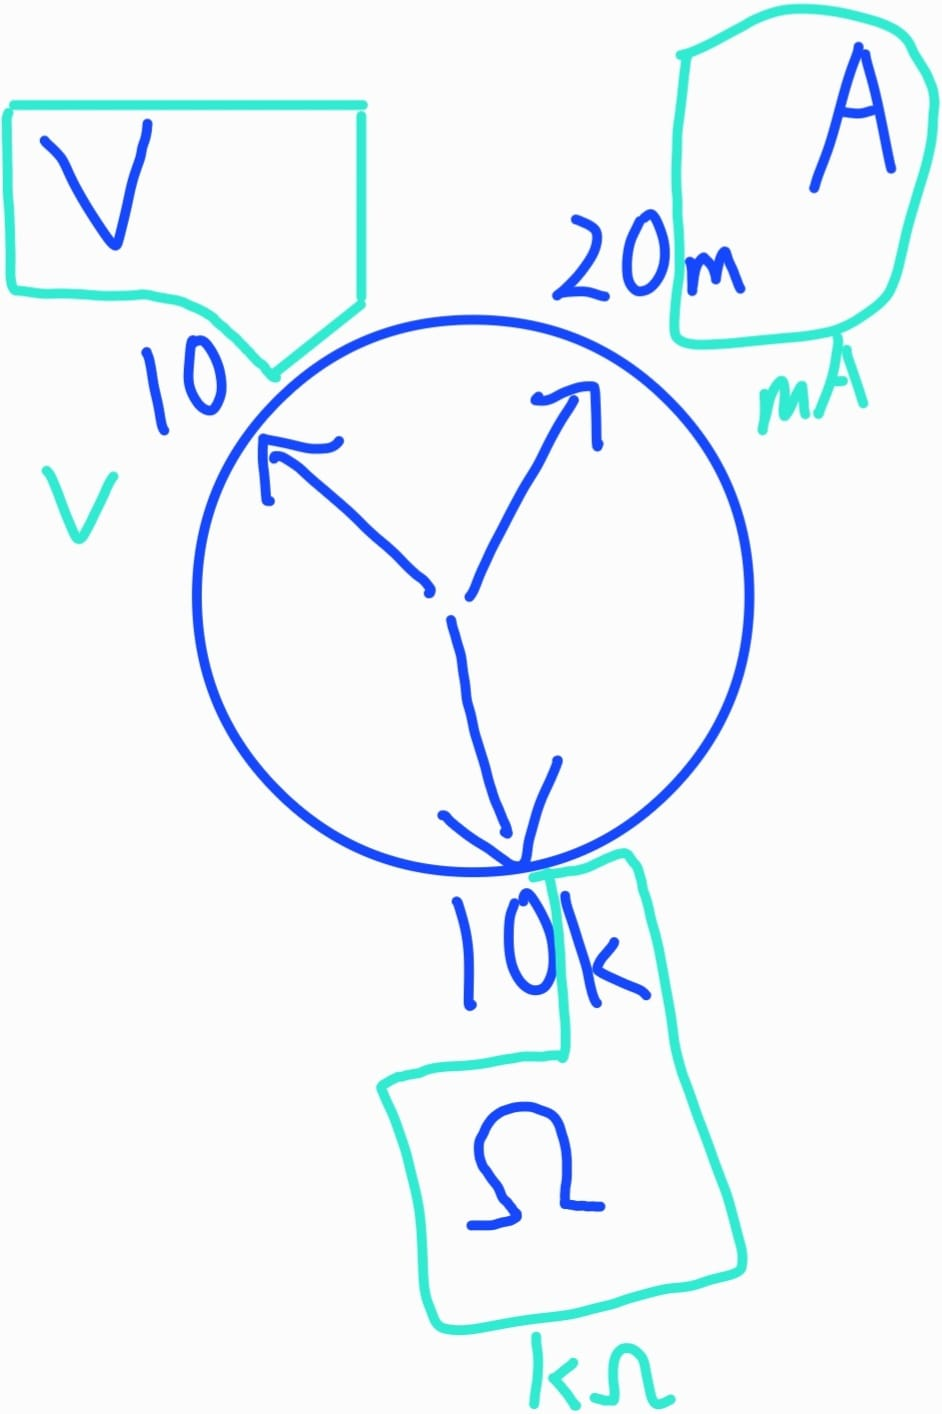
\includegraphics[width=0.3\textwidth]{../images/dmm-config.jpg}
        \caption{\ref{Me} The \textcolor{green!75!blue}{units} that a dmm is measuring in, given a \textcolor{blue}{particular config}.}
        \label{fig:dmm-config}
    \end{figure}
    \begin{figure}[H]
        \centering
        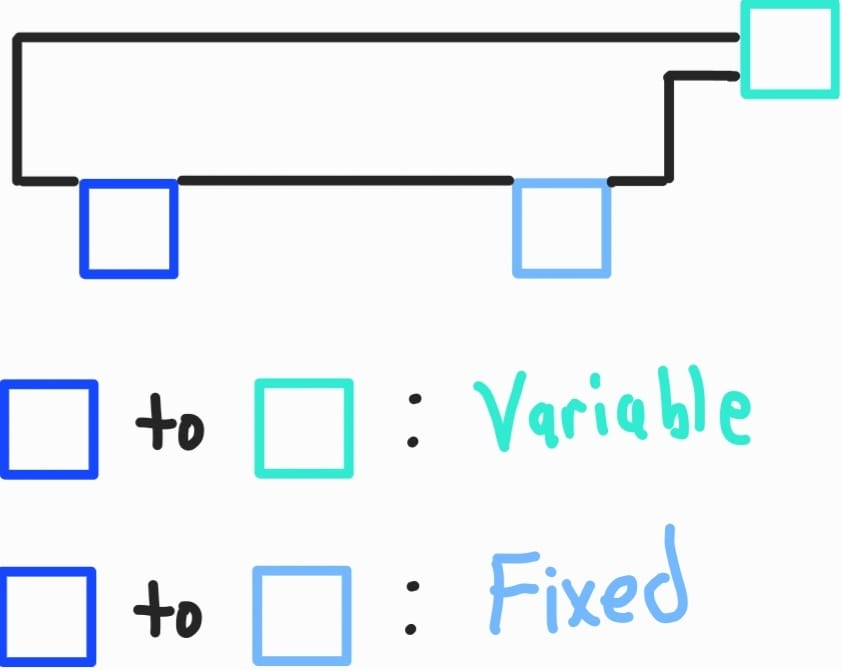
\includegraphics[width=0.3\textwidth]{../images/rheostat-config.jpg}
        \caption{\ref{Me} How to connect a rheostat to obtain a variable resistor or a fixed resistor.}
        \label{fig:rheostat-config}
    \end{figure}
        \item \emph{Accuracy} refers to \emph{how closely} a measured value \emph{agrees with its true value}.
        \item \emph{Precision} refers to \emph{how closely} individual measurements \emph{agree with each other}, without reference to a true value.
    \begin{table}[H]
        \centering
        \begin{tabular}{|Sc|Sc|Sc|Sc|Sc|}
            \hline
            \textbf{Instrument} & \textbf{Measurement} & \textbf{Readings} & \multicolumn{2}{Sc|}{\textbf{Precision of a measurement}}\\
            \hline
            \hline
            \textbf{Analogue Instruments} & \textbf{in general} & \textbf{2} & \multicolumn{2}{Sc|}{\textbf{smallest division}}\\ 
            \hline
            Metre rule & length & 2 & 0.1 cm & 1 mm\\
            \hline
            Vernier calipers & length & 2 & 0.01 cm & 0.1 mm\\
            \hline
            Micrometer screw gauge & length & 2 & 0.001 cm & 0.01 mm\\
            \hline
            \begin{minipage}{4cm}
                \centering
                Stopwatch\\
                (ensure \(t\geq 20\text{ s}\))
            \end{minipage} & time interval & 2 & \multicolumn{2}{Sc|}{
            \begin{minipage}{5cm}
                \centering
                0.01 s\\
                (but \(\Delta t=0.2-0.4\) s)
            \end{minipage}}\\
            \hline
            Thermometer & temperature & 2 & \multicolumn{2}{Sc|}{1 \(^\circ\)C}\\
            \hline
            Voltmeter & p.d. & 2 & \multicolumn{2}{Sc|}{smallest division}\\
            \hline
            Ammeter & current & 2 & \multicolumn{2}{Sc|}{smallest division}\\
            \hline
            Protractor & angle & 2 & \multicolumn{2}{Sc|}{\(1^{\circ}\)}\\
            \hline
            Measuring cylinder & volume & 1 & \multicolumn{2}{Sc|}{0.5 cm\(^3\)}\\
            \hline
            \hline
            \textbf{Digital instruments} & \textbf{in general} & \textbf{1} & \multicolumn{2}{Sc|}{
                \begin{minipage}{5cm}
                    \centering
                    \textbf{smallest increment displayed}\\
                    E.g. \(x=5.02\text{ g}\implies \Delta x=0.01\text{ g}\)
                \end{minipage}
            }\\
            \hline
        \end{tabular}
        \caption{The precision of some standard instruments.}
        \label{table:precision}
    \end{table}
    \begin{table}[H]
        \centering
        \begin{tabular}{|Sc|Sc|Sc|}
            \hline
            \multirow{2}{*}{\textbf{Operation}} & \multicolumn{2}{Sc|}{\textbf{D.P.\,/\,S.F.}}\\
            \cline{2-3}
            & Calculated value & Data used\\
            \hline
            \hline
            \multicolumn{3}{|Sc|}{\textbf{Addition and Multiplication}}\\
            \hline
            Addition & d.p. & least d.p.\\
            \hline
            Multiplication & s.f. & least s.f.\\
            \hline
            Multiplication by a fixed factor (e.g. \(\pi\)) & s.f. & s.f.\\
            \hline
            \hline
            \multicolumn{3}{|Sc|}{\textbf{Special Operations}}\\
            \hline
            Logarithms of base 10 or \(e\) & d.p. & s.f.\\
            \hline
            Trigonometric functions & s.f. & s.f.\\
            \hline
        \end{tabular}
        \caption{D.P.S.F.}
        \label{table:dpsf}
    \end{table}
    \begin{table}[H]
        \centering
        \begin{tabular}{|Sc|Sc|}
            \hline
            \textbf{Equation} & \textbf{Rules}\\
            \hline
            \(Z=aX\pm bY\) & \(\Delta Z=\lvert a \rvert\Delta X+\lvert b \rvert\Delta Y\)\\
            \hline
            \(Z=cX^aY^b\) & \(\dfrac{\Delta Z}{Z}=\lvert a \rvert\dfrac{\Delta X}{X}+\lvert b \rvert\dfrac{\Delta Y}{Y}\)\\
            \hline
        \end{tabular}
        \caption{Uncertainty rules}
        \label{table:uncertainty-rules}
    \end{table}
    \item Always take the average of three measurements (and show the working for the averaging explicitly) wherever possible. This reduces the effect of random error on the value of \rule{0.5cm}{0.05mm}\,, hence making it more precise.
    \item Always write the associated units for angles, be it \(\theta^{\circ}\) or \(\theta\) rad.
    \item After finishing calculations for a question, always check whether the number of s.f. or d.p. is correct. See table \ref{table:dpsf}.
    \item \emph{Note.} Whenever a physical quantity is given --- even a resistor clearly labelled ``\(10\Omega\)'' --- we still must account for its dpsf. However, if it's the number of turns/number of oscillations/etc, do not account for its dpsf.
    \item \emph{Note.} Even for physical constants --- such as \(e=1.60\cdot 10^{-19}\) --- their dpsf should also be taken into account! However, mathematical constants, like \(\pi\), can be disregarded in dpsf considerations. 
    \item In any set of repeated readings for time, the total time taken (e.g. for \(n\) oscillations) should not usually differ by more than human reaction time (\(0.2-0.4\)s).
    \item Percentage uncertainty of stopwatch,
    \[\frac{\Delta t}{t}=\frac{0.2}{\langle t \rangle}\cdot 100\%=\rule{0.5cm}{0.05mm}\,\%\ (1\ s.f.).\]
    \item Be careful of which quantities you are calculating. For example, in determining the radius \(r\) of an object, we might first measure its diameter \(d\). Take caution to remember to calculate \(r=d/2\), and \emph{not} carelessly write \(r=d\).  
    \item If it's difficult to measure a quantity accurately, we should account for it when calculating uncertainties. E.g. 
    \begin{enumerate}
        \item The base of a beaker is not flat. So its height \(h\) (measured with vernier calipers) has uncertainty \(\Delta h=0.2\) cm, rather than the usual \(0.01\) cm.
        \item It may be difficult to precisely measure the height \(h\) of a suspended object (with a metre rule). So, we use \(\Delta h=0.2\) cm, instead of the usual \(0.1\) cm. 
        \item It is difficult to maintain protraction when measuring an angle \(\theta\) (freehand) between, say, a metre rule and a string. Therefore, we account for this by taking \(\Delta\theta=3^\circ\), in place of the usual \(1^\circ\).
    \end{enumerate}
    In general, when expecting such sources of error, a safe bet is to take the absolute uncertainty to be twice the precision of the instrument. 
    \item Make the retort stands face inwards to increase stability
\end{itemize}
\section{Tables \& Graphing}
\begin{itemize}
    \item Define new variables --- i.e. ones that the question has not defined --- clearly. E.g. let \(n\) be the number of oscillations.
    \item Place all raw data on the left and leave space on the right to add extra columns.
    \item For the raw data for \(n\) oscillations, we can write it in this way:
    \begin{table}[H]
        \centering
        \begin{tabular}{|Sc|Sc|Sc|Sc|Sc|}
            \hline
            \(n\) & \(nT_1\)/s & \(nT_2\)/s & \(nT_3\)/s & \(T\)/s\\
            \hline
            &&&&\\
            \hline
        \end{tabular}
        \caption{Presentation of data for oscillations.}
        \label{table:raw-data-for-n-oscillations}
    \end{table} 
    % \item Ignore the dpsf of counting numbers, such as the number of oscillations \(n\). 
    \item Look out for
    \begin{enumerate}
        \item Correct column headings
        \item Dpsf of raw data
        \item Dpsf of calculated data
        \item Number of datasets (see Table \ref{table:practical-graph-points})
    \end{enumerate}
    \item The dependent variable is always plotted as the horizontal axis.
    \item Always include axis labels for every big square / every 2.0 cm.
    \item When drawing a best fit line, take note of the following:
    \begin{enumerate}
        \item The number of points above and below the line should differ by at most one.
        \item Do not draw a \textcolor{red}{`lopsided' graph}, as that is unlikely to be the \textcolor{green!70!black}{best fit line}.
        \begin{figure}[H]
            \centering
            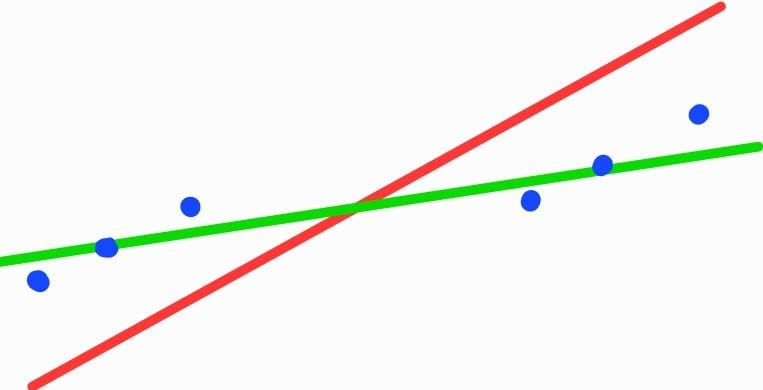
\includegraphics[width=0.3\textwidth]{../images/lopsided-best-fit-line.jpg}
            \caption{A \textcolor{red}{`lopsided' line} and the corresponding \textcolor{green!70!black}{best fit line}.}
            \label{fig:lopsided-best-fit-line}
        \end{figure}
    \end{enumerate}
    \item On anomalous points:
    \begin{table}[H]
        \centering
        \begin{tabular}{|Sc|Sc|Sc|}
            \hline
            Is there an anomalous point? & Graph & Anomaly statement\\
            \hline
            \textcolor{red}{\(\times\)} & Do nothing. &
            \begin{minipage}{0.7\textwidth-135.33138pt}
                There is no anomalous point as all plotted points follow the trend of the best fit line.
            \end{minipage}\\
            \hline
            \multirow{2}{*}[-3mm]{\textcolor{green!70!black}{\checkmark}} & 
            \multirow{3}{*}[-1mm]{
                \begin{minipage}{3.3cm}
                    Circle the point and write ``anomaly'' next to it.
                \end{minipage}
            } &
            \begin{minipage}{0.7\textwidth-135.33138pt}
                There is one anomalous point as it does not follow the trend of the best fit line.
            \end{minipage}\\
            \cline{3-3}
            &&
            \begin{minipage}{0.7\textwidth-135.33138pt}
                There is one anomalous point as it lies relatively far from the best fit line, \emph{compared to other points}.
            \end{minipage}\\
            \hline
        \end{tabular}
        \caption{Anomalous points.}
        \label{table:anomaly-statement}
    \end{table}
    \begin{table}[H]
        \centering
        \begin{tabular}{ScScSc}
            \toprule
            Type & Total number of points & Anomalous points allowed\\
            \midrule
            \multirow{2}{*}{Straight line} & 6 & 1\\
            & 7 & 2\\
            \midrule
            Curve & 8 & 1\\
            \bottomrule
        \end{tabular}
        \caption{Minimum number of points/maximum number of anomalous points.}
        \label{table:practical-graph-points}
    \end{table}
    \item Linearisation statement: 
    \begin{itemize}
        \item The equation can be rewritten as \(y=mx+c\). E.g. \(\frac{1}{L}=A+Ar\cdot\frac{1}{R_2}\).
        \item Plot \(y\) against \(x\). Then, if a straight best-fit line is obtained, the vertical intercept is \(c\) and the gradient is \(m\). 
    \end{itemize}
    \item Draw a gradient triangle using dotted lines and label the selected points (do not mark these points out using a dot/cross/etc).
    \item Always check that the two points selected for calculating gradient are stated to the correct number of decimal places, corresponding to half the smallest square.
    \item Follow the dpsf of the graph when calculating gradient. But follow the least sf of the graph and table when relating the gradient to a physical quantity.
    \begin{example}{}{}
        Consider when are given that \(y=mx+c\), where \(m\) and \(c\) are physical constants, and have the following table of values.
        \begin{table}[H]
            \centering
            \begin{tabular}{|Sc|Sc|Sc|Sc|}
                \hline
                \multirow{2}{*}{\(\cdots\)} & \(x\) & \(y\) & \multirow{2}{*}{\(\cdots\)}\\
                \cline{2-3}
                & (\(n_x\) s.f.) & (\(n_y\) s.f.) &\\
                \hline
            \end{tabular}
            \caption{The dpsf of the quantities \(x\) and \(y\).}
            \label{table:example-table-dpsf-gradient-physical-quantity}
        \end{table} 
        Suppose that, using values from our graph, \(y_2-y_1\) and \(x_2-x_1\) have \(m_y\) and \(m_x\) s.f., respectively. Then, 
        \[\text{gradient}=\frac{y_2-y_1}{x_2-x_1}=\rule{0.5cm}{0.01mm}\ (\min\{m_x,m_y\}\text{ s.f.})\]
        but
        \[a=\text{gradient}=\rule{0.5cm}{0.01mm}\ (\min\{n_x,n_y,m_x,m_y\}\text{ s.f.}).\]
    \end{example}
    \item Suppose we want to draw a new line such that its vertical intercept is the same as our best fit line, but our horizontal axis does not start from zero. Then, just ensure that the lines do not intersect.
\end{itemize}
\section{Questions post-graphing}
\begin{itemize}
    \item State/explain whether or not the results of your experiment supports the relationship that \rule{1cm}{0.05mm}\,.
    \[\text{Percentage difference}=\frac{k_{\text{larger}}-k_{\text{smaller}}}{k_{\text{larger}}}\cdot 100\%.\]
    \begin{itemize}
        \item Since the percentage difference of \(k=\rule{0.5cm}{0.05mm}\%>\rule{0.5cm}{0.05mm}\%={}\)the percentage uncertainty of \(\rule{0.5cm}{0.05mm}\)\,, the results of the experiment does not support the suggested relationship.
        \item Since the percentage difference of \(k=\rule{0.5cm}{0.05mm}\%\leq\rule{0.5cm}{0.05mm}\%={}\)the percentage uncertainty of \(\rule{0.5cm}{0.05mm}\)\,, the results of the experiment supports the suggested relationship.
    \end{itemize}
    \item Use your values in (f)(ii) to plot another point \(Z\) on your graph. State whether this point agrees with the pattern of the other points on your graph, with reference to your values in (a)(v) --- where we obtained two values for \(y\) (e.g. current \(I\)).
    \begin{itemize}
        \item Calculate the difference in current \(\Delta y_1\) between the \(y\) value obtained from the graph and the \(y\) value obtained in (f)(ii).
        \item Calculate half the range 
        \[\Delta y_2\coloneq\frac{y_{\text{higher}}-y_{\text{smaller}}}{2}\] 
        between the two values of \(y\) obtained in (a)(v).
        \item Since \(\Delta y_1> \Delta y_2\), this point \(Z\) does not agree with the pattern of the other points on the graph.
        \item Since \(\Delta y_1<\Delta y_2\), this point \(Z\) agrees with the pattern of the other points on the graph.
    \end{itemize}
    \item Avoid writing ``\dots because \rule{0.5cm}{0.05mm} is \textcolor{red}{not equal to} \rule{0.5cm}{0.05mm}''. Rather, we should say ``\dots because \rule{0.5cm}{0.05mm} is \textcolor{green!70!black}{far from/near to/close to} \rule{0.5cm}{0.05mm}''. 
    \item NY's suggested format for writing sources of error:
    \begin{itemize}
        \item What is error is/what causes the error, 
        \item Which raw data are affected.
    \end{itemize}
    An example. It is difficult to release the ball from the exact position (what the error is), as the ball is only released by a free hand, which is unsteady (what causes the error). This results in imprecise values of \(h\) (which raw data are affected).
    \item Examples of (i) significant sources of error and (ii) the ways to remedy them.
    % \begin{enumerate}
    %     \item[(a)(i)]  
    %     \item[(ii)]
    %     \item[(b)(i)] 
    %     % \begin{enumerate}[label=\arabic*.]
    %     %     \item 
    %     % \end{enumerate}
    %     \item[(ii)] 
    %     \item[(c)(i)] 
    %     \item[(ii)] 
    %     \item[(d)(i)] 
    %     \item[(ii)] 
    %     \item[(e)(i)] 
    %     \item[(ii)] 
    % \end{enumerate}
    \begin{longtable}{|Sc|Sc|}
        \hline
        \textbf{Source of error} & \textbf{Solution}\\
        \hline
        \hline
        \multicolumn{2}{|Sc|}{\textbf{RV J1 practical sessions}}\\
        \hline
        \begin{minipage}{0.5\textwidth-25.2pt}
            (J1 P01) It is difficult to maintain protraction, and hence, hard to measure \(\theta\) precisely.
        \end{minipage}&
        \begin{minipage}{0.5\textwidth-25.2pt}
            Clamp the protractor using another retort stand.    
        \end{minipage}\\
        \hline
        \begin{minipage}{0.5\textwidth-25.2pt}
            (J1 P04) There is significant friction between the hooks and the thread. (This adds systematic error into the measured values of \(t\).)
        \end{minipage}&
        \begin{minipage}{0.5\textwidth-25.2pt}
            Use rollers instead of hooks, to minimise the friction experienced by the moving thread.
        \end{minipage}\\
        \hline 
        \begin{minipage}{0.5\textwidth-25.2pt}
            (J1 P06) The values for current and voltage constantly fluctuate throughout the experiment. This introduces significant random error, which makes the value of \(c_2\) obtained less precise.
        \end{minipage}&
        \begin{minipage}{0.5\textwidth-25.2pt}
            Increase the mass of the oil added into the metal significantly. (So the measured values of \(t\) all increase in magnitude, reducing the effect of the random error\dots)
        \end{minipage}\\
        \hline
        \begin{minipage}{0.5\textwidth-25.2pt}
            (J1 P07)
        \end{minipage}&
        \begin{minipage}{0.5\textwidth-25.2pt}
            \begin{enumerate}[label=\arabic*.]
                \item Conduct the experiment using a sufficiently large hanger mass, such that the circular motion is more horizontal.
                \item Take a video of the experiment and analyse the data collected using tracking software.  
            \end{enumerate}
        \end{minipage}\\
        \hline
        \begin{minipage}{0.5\textwidth-25.2pt}
            (J1 P08) It is difficult to track the oscillating mass when the amplitude of the oscillations is small and the period is short.
        \end{minipage}&
        \begin{minipage}{0.5\textwidth-25.2pt}
            \begin{enumerate}[label=\arabic*.]
                \item Change the two springs to one equivalent spring of similar effective spring constant.
                \item Use a heavier mass but which does not cause the springs to exceed their limit of proportionality.
                \item Provide a visual mark near the oscillating mass to help in tracking its movement.
            \end{enumerate} 
        \end{minipage}\\
        \hline
        \hline
        \multicolumn{2}{|Sc|}{\textbf{RV J2 practical sessions}}\\
        \hline
        \begin{minipage}{0.5\textwidth-25.2pt}
            (J2 P04) The precise point where resonance occurs is not easily determined when the vibration of the wire is not significant enough to be observed.
        \end{minipage}& 
        \begin{minipage}{0.5\textwidth-25.2pt}
            \begin{enumerate}
                \item Increase the magnetic flux density by using a stronger magnet, e.g. neodymium magnets.
                \item Add a white grid (e.g. graph paper) behind the wire, so that it is easier to estimate and compare the magnitude of oscillation.
            \end{enumerate}
        \end{minipage}\\
        \hline
        \begin{minipage}{0.5\textwidth-25.2pt}
            (J2 P06)
            \begin{enumerate}
                \item It is hard to ensure that the oscillation is only about the vertical axis. Moreover, the ruler tends to swing back and forth, affecting the measurement of \(T\).
                \item It is hard to measure the angle freehand using a protractor without disturbing the equilibrium of the system.
            \end{enumerate}
        \end{minipage}&
        \begin{minipage}{0.5\textwidth-25.2pt}
            \begin{enumerate}
                \item Keeping the ruler in the horizontal position will make it rotate more easily about the vertical axis.
                \item Secure the protractor to another retort stand, so that the protractor can be brought near to the system to read off the angle.
            \end{enumerate}
        \end{minipage}\\
        \hline
        \hline
        \multicolumn{2}{|Sc|}{\textbf{NY practicals}}\\
        \hline
        \begin{minipage}{0.5\textwidth-25.2pt}
            The large size of the object resulted in a larger uncertainty in the measurement.
        \end{minipage}& 
        Use a thinner/smaller object\\
        \hline
        \begin{minipage}{0.5\textwidth-25.2pt}
            The mark is larger than the smallest division of \rule{0.5cm}{0.05mm}.
        \end{minipage}&
        Use a smaller mark.\\
        \hline
        \begin{minipage}{0.5\textwidth-25.2pt}
            It is difficult for the naked eye to pinpoint the exact moment when the object crosses the mark. 
        \end{minipage}&
        \begin{minipage}{0.5\textwidth-25.2pt}
            Take a video of the experiment. Then, using tracking software, find the exact time when the object crosses the mark. 
        \end{minipage}\\
        \hline
        \begin{minipage}{0.5\textwidth-25.2pt}
            (Experiment 01)
            \begin{enumerate}
                \item Human reaction time.
                \item The rubber band is thicker than the smallest division of the ruler used and this adds error to the measured values of \(s\).
            \end{enumerate}
        \end{minipage}& 
        \begin{minipage}{0.5\textwidth-25.2pt}
            \begin{enumerate}
                \item Place two photogates, held by retort stands, at [location of gates]. Then, connect both photogates to an electronic timer. We use this photogates set-up to start and stop the measurement of the time \(t\).
                \item Replace the rubber band with a brightly coloured thin string and tie a loop around the cylinder.
            \end{enumerate}
        \end{minipage}\\
        \hline
        \begin{minipage}{0.5\textwidth-25.2pt}
            (Experiment 02) One's hand is not steady and cannot release the object from the same velocity/position consistently.
        \end{minipage}& 
        \begin{minipage}{0.5\textwidth-25.2pt}
            Use a ruler/retort stand/etc to hold the object in a stable position before release so the initial velocity is constant.
        \end{minipage}\\
        \hline
        \begin{minipage}{0.5\textwidth-25.2pt}
            (Experiment 05) The upper string might not be parallel to the ground as it is just an estimate by the human eye. Hence, the value of \(h\) would be inaccurate.
        \end{minipage}&
        \begin{minipage}{0.5\textwidth-25.2pt}
            A ruler and a set square can be used to ensure that the string is perpendicular to the retort stand, which is perpendicular to the tabletop. Hence, this makes the values of \(h\) more accurate.
        \end{minipage}\\
        \hline
        \begin{minipage}{0.5\textwidth-25.2pt}
            (Experiment 07) 
            \begin{enumerate}
                \item It is difficult to ascertain the extreme position of the ball accurately as it is only at rest instantaneously. This results in imprecision.
                \item It is difficult to release the ball with constant height.
            \end{enumerate}
        \end{minipage}&
        \begin{minipage}{0.5\textwidth-25.2pt}
            \begin{enumerate}
                \item Use of a motion sensor/video.
                \item Use of a release mechanism.
            \end{enumerate}
        \end{minipage}\\
        \hline
        \begin{minipage}{0.5\textwidth-25.2pt}
            (Experiment 13) Kinks in the wire.
        \end{minipage} & 
        \begin{minipage}{0.5\textwidth-25.2pt}
            Use a wingbolt to tighten the wire.
        \end{minipage}\\
        \hline
        \begin{minipage}{0.5\textwidth-25.2pt}
            (Experiment 15) The paper cone is flimsy and cannot hold a perfect circular shape at the base of the cone. Hence, this causes the values at \(\theta\) to be smaller than expected. So, precision is lost for the values of \(h\), \(y\), and \(x\).
        \end{minipage}&
        \begin{minipage}{0.5\textwidth-25.2pt}
            Use a plastic cone, so that the measurements for \(h\), \(x\), and \(y\) are more precise, as the shape of the cone cannot change.
        \end{minipage}\\
        \hline
        % \begin{minipage}{0.5\textwidth-25.2pt}
            
        % \end{minipage}&
        % \begin{minipage}{0.5\textwidth-25.2pt}
            
        % \end{minipage}\\
        % \hline
    \caption{Additional examples of sources of errorrs and the corresponding solutions.}
    \label{table:sources-of-error-and-solutions}
    \end{longtable}
\end{itemize}
\section{Planning questions}
\begin{table}[H]
    \centering
    \begin{tabular}{|Sc|Sc|}
        \hline
        Context & Sentence\\
        \hline
        \begin{minipage}{0.5\textwidth-25.2pt}
            A solar panel heats water by absorbing intra-red radiation from the Sun. It consists of an array of pipes, through which water is passed\dots Design an experiment to determine the efficiency of a model solar panel.
        \end{minipage}&
        \begin{minipage}{0.5\textwidth-25.2pt}
            Check that there is a significant temperature difference between the two thermometers. If not, adjust the power of the lamp. This will help us to determine the range of suitable values of intensity that can be used.
        \end{minipage}\\
        \hline
        \begin{minipage}{0.5\textwidth-25.2pt}
            The efficiency of a motor is thought to depend on the angular velocity \(\omega\) of the motor. The relation between the efficiency and the angular velocity \(\omega\) of the motor may be written in the form \(\eta=a\omega^b\), where \(a\) and \(b\) are constants\dots
        \end{minipage}&
        \begin{minipage}{0.5\textwidth-25.2pt}
            Check for the appropriate masses and heights such the mass can be raised when adjusting the angular speed of the motor using the variable power supply.
        \end{minipage}\\
        \hline
    \end{tabular}
    \caption{Examples on preliminary readings.}
    \label{table:preliminary-readings}
\end{table}
\begin{itemize}
    \item For \emph{short} planning questions, we can reference the question's diagram(s). But we must include \emph{our own} for \emph{long} planning questions.
    \item Always include a bench to avoid floating equipment.
    \item In testing for a linear relationship, we must state that the best fit line should be a \emph{straight line}. If we're testing for direct proportionality, this line should also \emph{cut through the origin}. 
    \item A ``\(\circ\)''  denotes a point outside of accuracy/precision/safety precautions.
    \begin{longtable}{M{0.1\textwidth}m{0.4\textwidth}m{0.4\textwidth}}
        \toprule
        Topic & \centering Accuracy/Precision & \centering Safety
        \tabularnewline\midrule
        General &
        \begin{itemize}
            \item[\textcolor{green!70!black}{\checkmark}] Always take preliminary readings.
            \item[\textcolor{green!70!black}{\checkmark}] Measure \(t\) thrice and take the average.
            \item[\textcolor{green!70!black}{\checkmark}] Remove all other sources of \rule{1cm}{0.01mm} (sound/light/etc) before conducting the experiment, to reduce systematic/random error. \hyperlink{error:other-sources-of-alternating-magnetic-fields}{(circuits e.g.)} \hyperlink{error:other-sources-of-sound}{(sound e.g.)}
        \end{itemize}
        &
        \tabularnewline\midrule
        Nuclear & 
        \begin{itemize}
            \item[\textcolor{green!70!black}{\checkmark}] Preliminary readings. E.g. Determine the range of distances \(d\) and thicknesses \(t\) of front plates that will give a measurable difference in the count rate. 
            \item[\textcolor{green!70!black}{\checkmark}] Repeat the measurements for \(C_b\) and \(C_T\) thrice and take the average.
            \item[\textcolor{green!70!black}{\checkmark}] Measure the background count rate \(C_b\) and subtract it from the total count rate \(C_T\), to obtain the count rate \(C=C_T-C_b\) of the sample.   
        \end{itemize}
        &
        \begin{itemize}
            \item[\textcolor{green!70!black}{\checkmark}] The source is handled with a pair of tongs, to prevent contact with the radioactive material.
            \item[\textcolor{green!70!black}{\checkmark}] The source is stored in a lead lined box when not in use, to prevent contact with the radioactive material.
            \item[\textcolor{green!70!black}{\checkmark}] Cordon off the area with tape and put up a warning sign, to prevent others from being exposed to radioactive material. 
            \item[\textcolor{red}{\(\times\)}] Avoid pointing the source at people.
            \item[\textcolor{red}{\(\times\)}] Do not look directly at the source.
            \item[\textcolor{red}{\(\times\)}] Protective clothing, lead suits, lead gloves, goggles.   
        \end{itemize}
        \tabularnewline\midrule
        Thermal &
        \begin{itemize}
            \item[\textcolor{green!70!black}{\checkmark}] Check calibration of thermometer (mercury-in-glass/temperature sensor) against melting pure ice and pure steam.
            \item[\textcolor{green!70!black}{\checkmark}] A constant temperature environment can be set up using a sand bath, water bath, or putting the object into an oven.
            \item[\textcolor{green!70!black}{\checkmark}] Enclose the object to prevent convection currents from forming in the air.   
            \item[\(\circ\)] Connect the thermocouple to a voltmeter. Calibrate The thermocouple by placing one junction of the thermocouple into water at ice point (pure ice-water mixture) and the other into steam point (boiling pure water). Allow the voltage to stabilise and record the voltage reading as \(V_0\). Remove the junction at steam point and place it on the \rule{1cm}{0.01mm}. Record the voltage reading as \(V\). Then,
            \[T=\frac{V}{V_0}\cdot100\ {^{\circ}C}.\] 
            \item[\(\circ\)] Place the temperature sensor in the \rule{1cm}{0.01mm}. Connect the temperature sensor to a datalogger and computer to generate a graph of temperature against time.
        \end{itemize}
        &
        \begin{itemize}
            \item[\textcolor{green!70!black}{\checkmark}] Wear heat insulating gloves.
            \item[\textcolor{green!70!black}{\checkmark}] Avoid touching the hot objects.
        \end{itemize}
        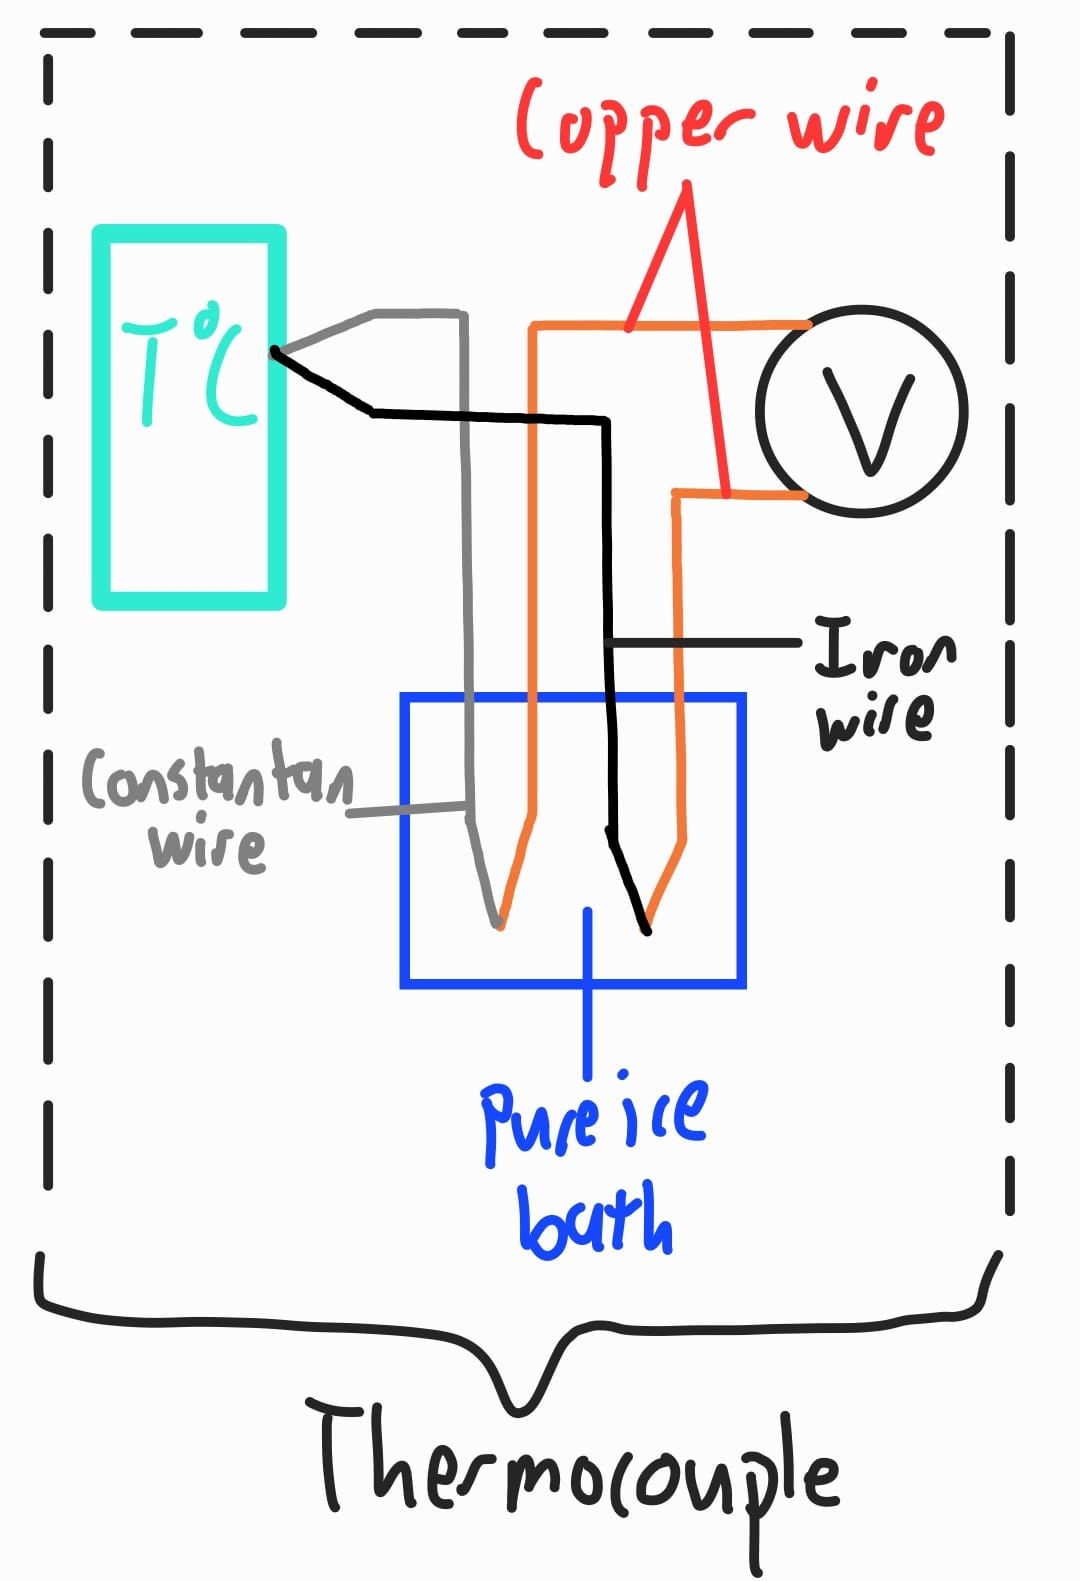
\includegraphics[width=\linewidth]{../images/thermocouple-planning-diagram.jpg}
        \tabularnewline\midrule
        \newpage\midrule
        Waves &
        \begin{itemize}
            \item Sound
            \begin{itemize}
                \item[\textcolor{green!70!black}{\checkmark}] \hypertarget{error:other-sources-of-sound}{Conduct the experiment in a soundproofed room, to minimise random error due to environmental noise.}   
            \end{itemize} 
        \end{itemize}   
        &
        \begin{itemize}
            \item Light
            \begin{itemize}
                \item[\textcolor{green!70!black}{\checkmark}] Do not look directly at the light source, or point it directly at anyone.
                \item[\textcolor{green!70!black}{\checkmark}] Wear a pair of laser safety glasses (or shades for non-lasers) to protect the eyes.
                \item[\textcolor{green!70!black}{\checkmark}] Wear heat insulating gloves when moving the hot light source.  
            \end{itemize}
            \item Sound
            \begin{itemize}
                \item[\textcolor{green!70!black}{\checkmark}] Wear ear muffs to prevent hearing damage.
                \item[\textcolor{green!70!black}{\checkmark}] Switch on the sound source for a short period of time; turn it off when the apparatus is not in use.
            \end{itemize}
        \end{itemize}
        \tabularnewline\midrule
        Mechanics &
        \begin{itemize}
            \item[\textcolor{green!70!black}{\checkmark}] Explain clearly how to find the frequency of vibration \(f\). 
            
            Starting with the highest available frequency, the frequency of strobing is gradually reduced till the vibrating object appears stationary. Record the frequency of vibration \(f\) as the frequency of strobing.  
            \item[\textcolor{green!70!black}{\checkmark}] Explain clearly how to use a pair of photogates with an electronic timer to obtain the time taken \(t\).
    
            The object is projected so that it passes through both photogates. Record the times at which it passes through each gate as \(t_1\) and \(t_2\). Calculate the time taken \(t=t_2-t_1\).
            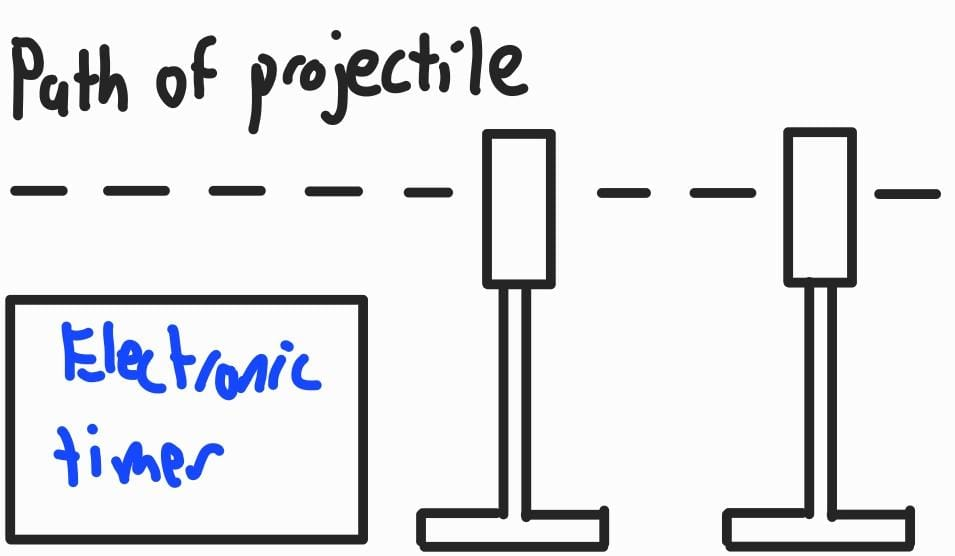
\includegraphics[width=\linewidth]{../images/electronic-timer-light-gates.jpg}
            When the distance between the gates is small, the average velocity\({}\approx{}\)instantaneous velocity.
        \end{itemize}
        & 
        \begin{itemize}
            \item Water/oil
            \begin{itemize}
                \item[\textcolor{green!70!black}{\checkmark}] Mop up any spillage of oil/water to avoid injuries due to falling.
            \end{itemize}
            \item Load
            \begin{itemize}
                \item[\textcolor{green!70!black}{\checkmark}] Wear safety boots to reduce possible injuries to your feet.
            \end{itemize}
            \item Moving parts
            \begin{itemize}
                \item[\textcolor{green!70!black}{\checkmark}] Avoid the moving blades of the fan using a safety screen. Switch off the fan when the apparatus is not in use. 
            \end{itemize}
            \item Glass
            \begin{itemize}
                \item[\textcolor{green!70!black}{\checkmark}] Wear thick safety googles and thick gloves to prevent injury when handling the glass.
            \end{itemize}
        \end{itemize}
        \tabularnewline\midrule
        \newpage\midrule
        E\&M &
        \begin{itemize}
            \item[\textcolor{green!70!black}{\checkmark}] Preliminary readings. E.g. Determine the range of frequencies \(f\) of e.m.f. and cross sectional area of the coil \(X\) that lead to a measurable range of induced e.m.f. \(\varepsilon\).
            \item[\textcolor{green!70!black}{\checkmark}] Use an iron core to increase the e.m.f. induced.
            \item[\textcolor{green!70!black}{\checkmark}] Detailed description on how to use the cathode ray oscilloscope (c.r.o.) to obtain raw data. E.g. 
            \begin{enumerate}
                \item Using the grid on the screen, measure the maximum vertical distance \(y\) occupied by a complete waveform. Multiply \(y\) by the scale indicated on the \(Y\)-gain to obtain the peak voltage \(V_0\).
                \item Using the grid on the screen, measure the horizontal distance \(x\) occupied by a complete waveform. Multiply \(x\) by the scale indicated on the time base to obtain the period \(T\).
            \end{enumerate}
            (The c.r.o. should be connected in parallel for the above.)
            \item[\textcolor{green!70!black}{\checkmark}] \hypertarget{error:other-sources-of-alternating-magnetic-fields}{Remove all other sources of alternating magnetic fields, which lead to systematic error, before starting the experiment.}
            \item[\textcolor{green!70!black}{\checkmark}] Connect a Hall probe to a Gaussmeter. Calibrate the probe using a magnetic field of known strength. Then, orient the hall probe till a maximum voltage reading \(V_0\) is obtained. Repeat this a few times at different positions; the magnetic field is uniform if \(V_0\) remains approximately constant. 
        \end{itemize} 
        & 
        \begin{itemize}
            \item[\textcolor{green!70!black}{\checkmark}] Wear rubber gloves.
            \item[\textcolor{green!70!black}{\checkmark}] Switch off the power supply when the apparatus is not in use to avoid overheating the wire/coil/etc. 
            \item[\textcolor{green!70!black}{\checkmark}] Do not touch the coil because might be hot.
            \item[\textcolor{red}{\(\times\)}] Do not mention electric shocks when the current and voltage used are small.  
            
            \vspace{9.5cm}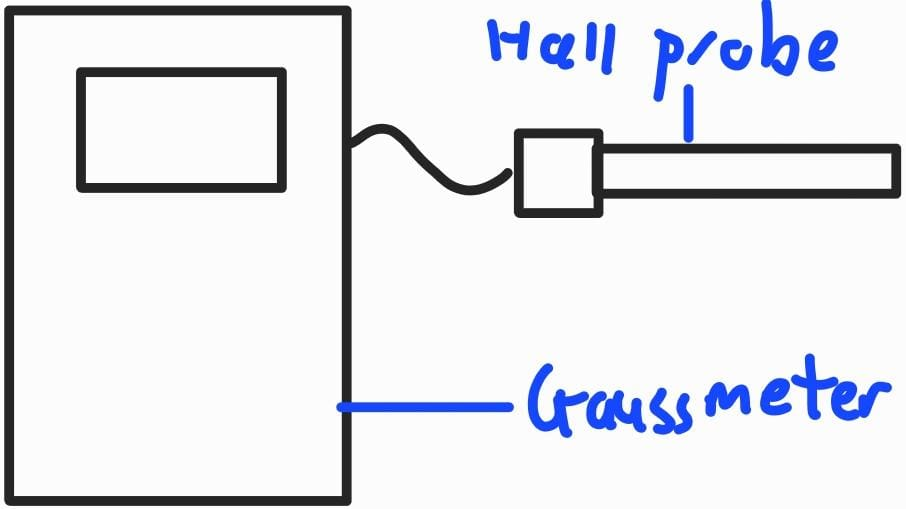
\includegraphics[width=\linewidth]{../images/gaussmeter-Hall-probe.jpg}
        \end{itemize}
        \tabularnewline
        &
        \begin{itemize}
            \item[\(\circ\)] Specify which setting, d.c. or a.c., an ammeter or voltmeter should be used in.
            \item[\(\circ\)] A c.r.o. can either be connected directly to an electrical circuit, or to a microphone. 
            \item[\(\circ\)] A signal generator is an a.c. source with variable frequency, amplitude, and waveform. It can be connected to a loudspeaker.
        \end{itemize}
        \vspace{1.2cm}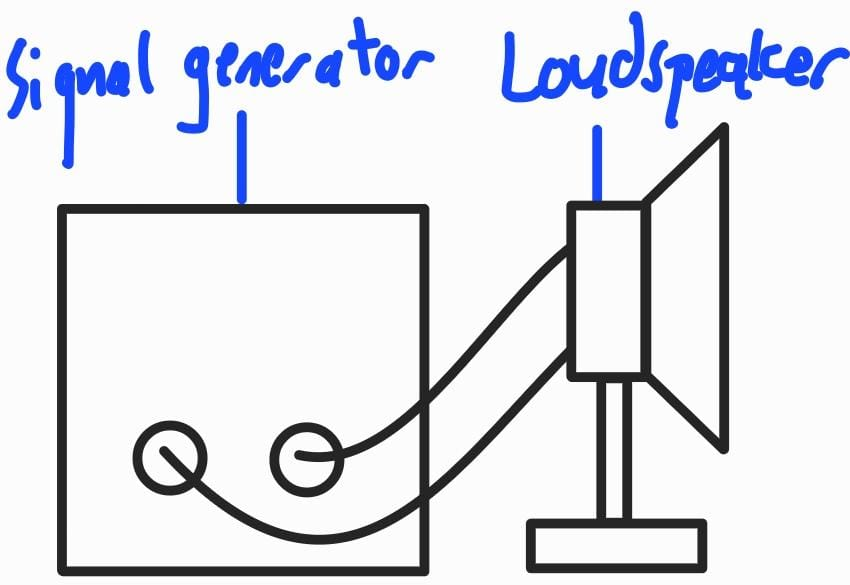
\includegraphics[width=\linewidth]{../images/signal-gen-loudspeaker.jpg}
        &
        \begin{minipage}{\linewidth}
            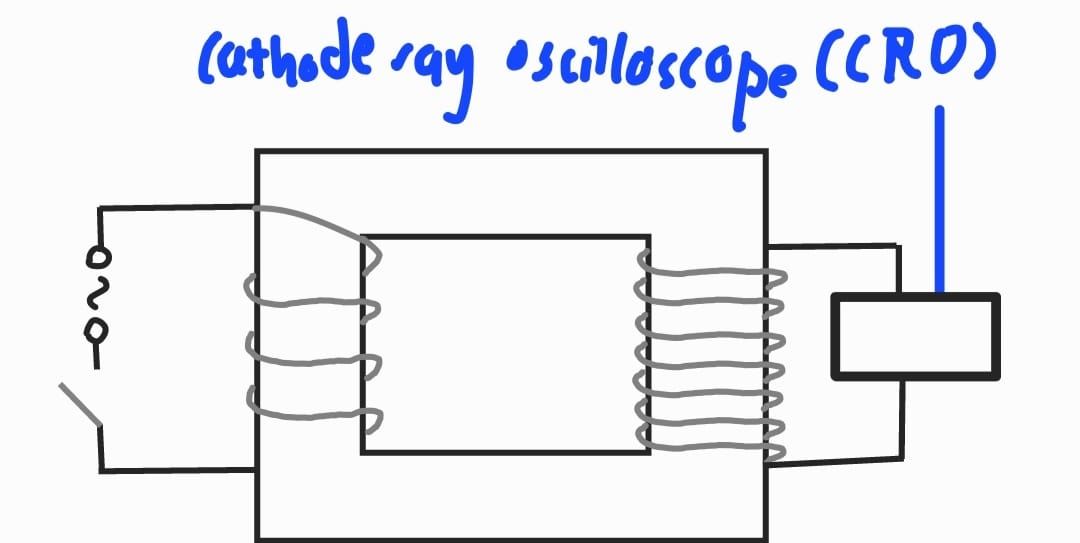
\includegraphics[width=\linewidth]{../images/cro-transformer.jpg}\\
            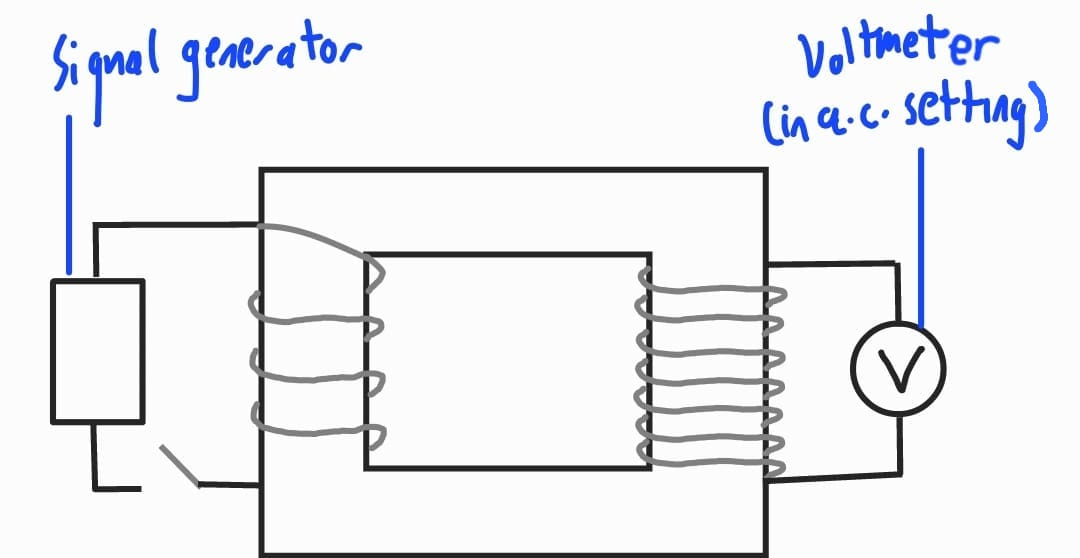
\includegraphics[width=\linewidth]{../images/signal-gen-voltmeter-transformer.jpg}\\
            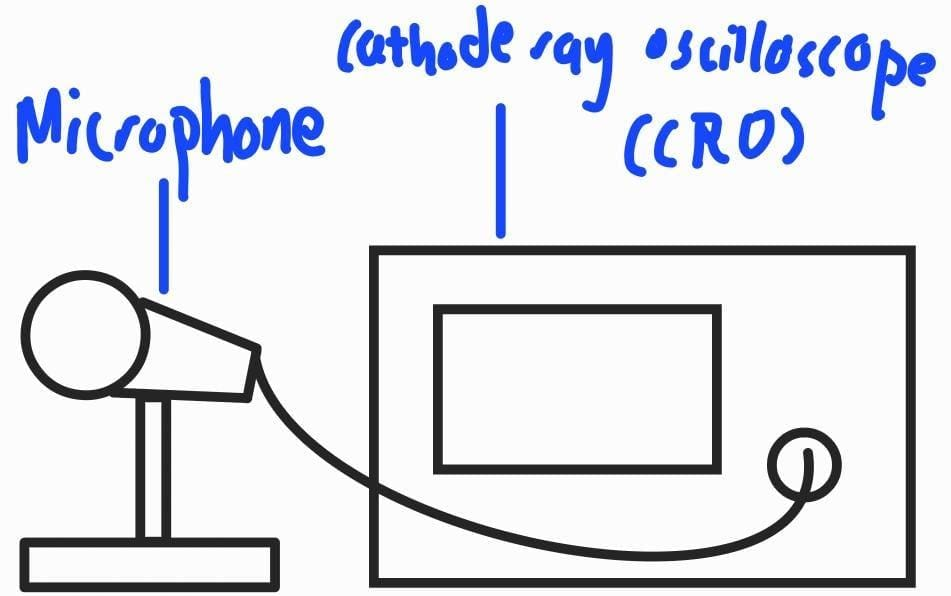
\includegraphics[width=\linewidth]{../images/cro-mic.jpg}\\
        \end{minipage}%
        \tabularnewline%
        &
        \begin{itemize}
            \item A uniform magnetic field can be produced using a Helmholtz coil. If necessary, a hall probe can be placed, perpendicular to the magnetic field/perpendicular to the plane of the paper.
        \end{itemize}
        &
        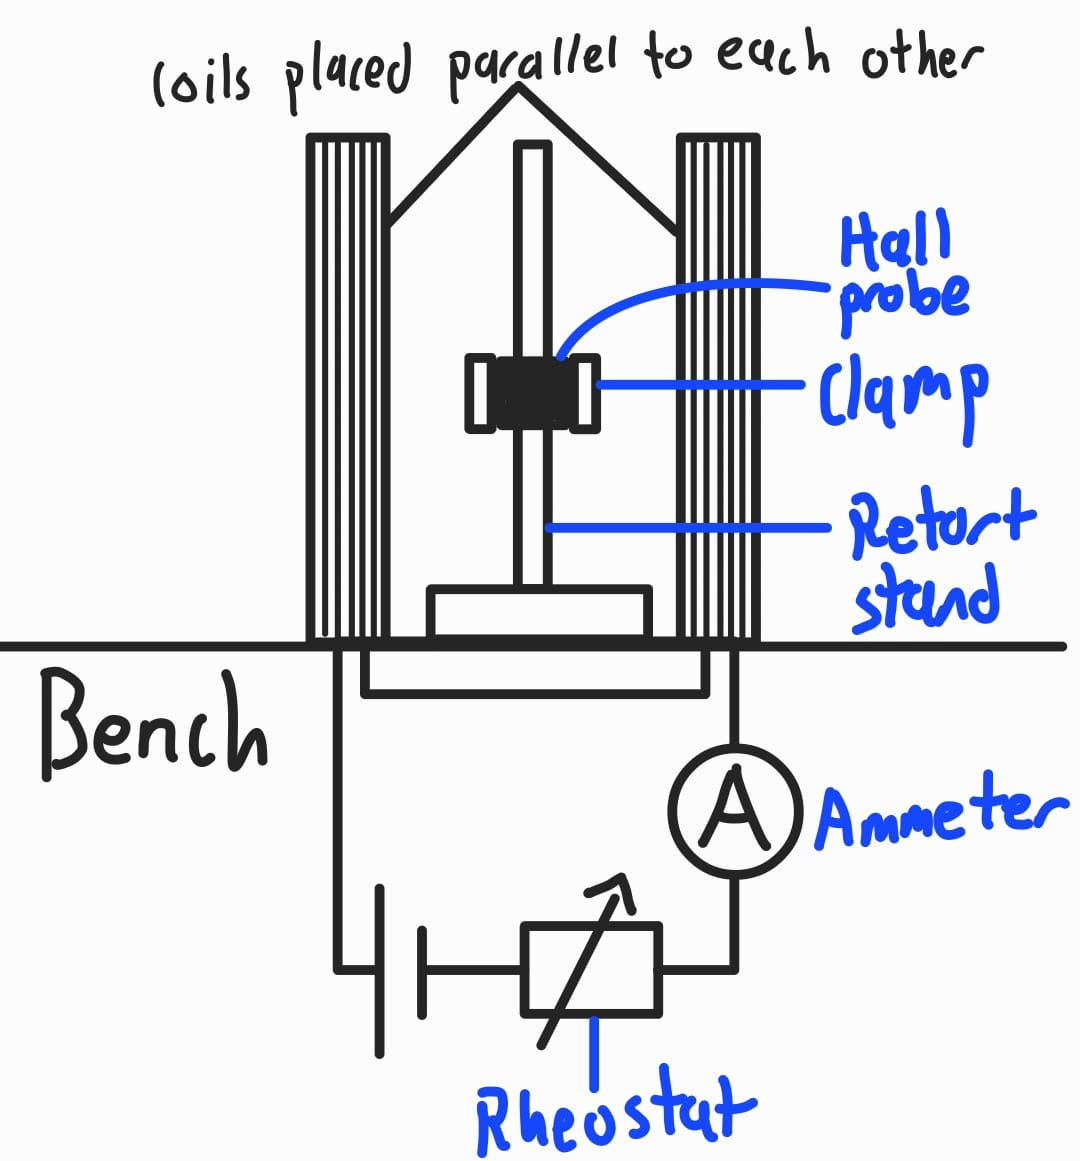
\includegraphics[width=\linewidth]{../images/Helmholtz-coil.jpg}
        \tabularnewline\bottomrule
        \caption{Precautions and some miscellaneous notes.}
        \label{table:precautions}
    \end{longtable}
\end{itemize}
(All figures in table \ref{table:precautions} are attributed to \ref{Me}.)
\begin{figure}[H]
    \centering
    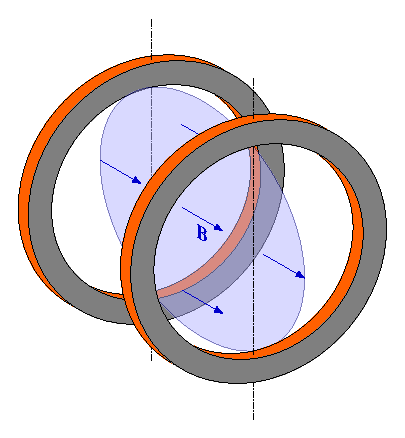
\includegraphics[width=0.7\textwidth]{../images/Helmholtz-Coil/coil.pdf}
    \caption{\ref{source:Helmholtz-Coil} A Helmholtz coil.}
    \label{fig:Helmholtz-Coil}
\end{figure}
\begin{itemize}
    \item Other instruments to know: newton meter, flow rate meter (\(dV/dt\)), mass flow meter \((dm/dt)\), pressure gauge, light intensity meter, sound level meter.
\end{itemize}